\chapter{Moving into $\RR^3$}\label{chap:moving-into-r3}
\setlength\epigraphwidth{.9\textwidth}
\epigraph{The wild things roared their terrible roars and gnashed their terrible teeth\\
  and rolled their terrible eyes and showed their terrible
  claws}{---Maurice Sendak, \emph{Where the Wild Things Are}}


In this chapter, we partially extend the machinery from the previous
chapter for use in $\RR^3$. The idea is that away from crossing
points, arcs in our diagrams in $\RR^2$ can just be treated with
\cref{thm:bounded-arcs-with-same-endpoints}, and this lifts to an
ambient isotopy in $\RR^3$ that only affects one strand. We will use
this in developing a simple condition on our diagrams that guarantees
we can represent the corresponding embeddings by countable unions of
polygonal segments --- namely, that the set of crossing points are
topologically discrete. In addition to tame arcs, certain classes of
wild arcs (e.g., the Fox-Artin curve in \cref{ex:fox-artin-curve})
will fall into this category. This sets the stage for future work in
which we hope to use \cref{thm:uniformly-convergent-ambient-isotopy}
to show an analogue of Reidemeister's theorem holds. We present a
sketch of how we might plan to attack the problem, however, we have
not confirmed the details. % {\color{blue} !!!!!!!!}

We begin by defining a slightly-relaxed version of regular diagrams,
namely \emph{discrete diagrams}. These are identical to regular
diagrams, except we allow the set of crossing points to be
\emph{discrete} instead of restricting them to be \emph{finite}. Note,
the discreteness condition allows at most countably-many crossings
(\cref{prop:at-most-countable-crossings}).

In \cref{sec:controlling-behavior-away-from-crossings} and
\cref{sec:controlling-behavior-near-crossings}, we then develop the
two pieces of machinery needed to analyze such diagrams.
\cref{sec:controlling-behavior-away-from-crossings} is concerned with
demonstrating that planar isotopy is \emph{always} valid, even without
PL constraints. This allows us to control the behavior of our knots
away from crossings, and the proofs are fairly straightforward in
light of \cref{chap:ambient-isotopy-in-r2}. In
\cref{sec:controlling-behavior-near-crossings}, we do the
complimentary analysis, showing we can control the behavior of our
knots near crossing points; in particular, we can represent every
crossing by two perpendicular line segments.\footnote{Of course, this
  might seem obvious, but a rigorous argument turns out to be highly
  technical given that we are \emph{only} assuming the crossings are
  discrete (and not that our knot is tame).}

Finally, we put these pieces together to yield the promised proof that
a discrete diagram is sufficient to guarantee a representation as a
countable union of polygonal segments. Anyways, the definition.

\begin{definition}[Discrete Diagram]
  Let $K : S^1 \into \RR^3$ be an embedding. Let $\pi : \RR^3 \to
  \RR^2$, and let $D$ be the diagram of $K$ given by $\pi$. Then we
  say $D$ is a \emph{discrete} diagram iff
  \begin{enumerate}
    \item (No multi-crossings): For all $p \in D$,
      $\abs{\fpre{\pi}{p}} \leq 2$
    \item (All crossings are transverse): The diagram is locally
      $X$-shaped at points of crossing, and
    \item (Crossings are discrete): The set $\ms C$ of crossing points
      of $D$ is topologically discrete in $\RR^2$. \qedhere
  \end{enumerate}
\end{definition}
We have the following proposition:
\begin{proposition}\label{prop:at-most-countable-crossings}
  If $D$ is a discrete diagram, then the set of crossing points $\ms
  C$ is at most countable.
\end{proposition}
\begin{sproof}
  $\ms C$ is a subspace of $\RR^2$, which is second-countable. It
  follows $\ms C$ is second-countable. Since a discrete space is
  second-countable iff it is countable, we have the desired result.
\end{sproof}

One might wonder what a \emph{non}-discrete diagram might look like,
and whether it is even possible to obtain one. Indeed we can ---
\emph{everywhere-wild} knots are examples of embeddings for which no
diagram is discrete. We provide an example construction below (imagine
taking the limit as $n \to \infty$), but for more on this subject, one
should reference \cite{Shilepsky} and \cite{Bothe1981}.
\begin{figure}[H]
  \centering
  \includegraphics[scale=.3]{figures/infinite-gauss-sequence/test/test-0.pdf}
  \caption{Step 1 in the construction of an everywhere-wild knot}
\end{figure}
\begin{figure}[H]
  \centering
  \includegraphics[scale=.3]{figures/infinite-gauss-sequence/test/test-1.pdf}
  \caption{Step 2 in the construction of an everywhere-wild knot}
\end{figure}
\begin{figure}[H]
  \centering
  \includegraphics[scale=.5]{figures/infinite-gauss-sequence/test/test-2.pdf}
  \caption{Step 3 in the construction of an everywhere-wild knot}
  \label{fig:everywhere-wild-3}
\end{figure}
% Another example comes from the following, which is similar to the
% construction for the koch snowflake.
% \begin{figure}[H]
%   \centering
%   \includegraphics[scale=.1]{figures/rectifiable-knots/koch-knot-0.pdf}
%   % \caption{Step 1 in the construction of an everywhere-wild knot}
% \end{figure}
% \begin{figure}[H]
%   \centering
%   \includegraphics[scale=.1]{figures/rectifiable-knots/koch-knot-1.pdf}
%   % \caption{Step 2 in the construction of an everywhere-wild knot}
% \end{figure}
% \begin{figure}[H]
%   \centering
%   \includegraphics[scale=.1]{figures/rectifiable-knots/koch-knot-2.pdf}
%   % \caption{Step 3 in the construction of an everywhere-wild knot}
%   % \label{fig:everywhere-wild-3}
% \end{figure}





% \begin{figure}[H]
%   \centering
%   \begin{tikzpicture}[scale=.75]
%     % Define the radii of our nested circles
%     \pgfmathsetmacro{\ra}{2} % Biggest
%     \pgfmathsetmacro{\rb}{3} % Medium
%     \pgfmathsetmacro{\rc}{4} % Small

%     % How much spacing in $x$ to put between the circles
%     % \pgfmathsetmacro{\xsep}{10cm}
%     \begin{scope}
%       \foreach \r/\n in {
%         \ra/.2, \rb/.1, \rc/0
%       }{ % Draw the circles first so that they don't cross
%         % with the arrows
%         \draw ($(0, \r) + (0, \n)$) circle (\r cm);
%         \draw ($(10, \r) + (0, \n)$) circle (\r cm);
%       }

%       \foreach \r/\n/\llab/\rlab in {
%         \ra/.2/$F(K)$ polygonal/$C_D$ is finite,
%         \rb/.1/$F(K)$ rectifiable/$C_D$ is discrete,
%         \rc/0/$F(K)$ is a knot/$C_D$ is disconnected
%       }{
%         % Where to draw the node label
%         \pgfmathsetmacro{\nodey}{2*\r - \ra/2}

%         \node (\r k) at (0, \nodey) {\llab};
%         \node (\r d) at (10, \nodey) {\rlab};

%         \begin{scope}[transform canvas={yshift=.3em}]
%           \draw[-implies, double equal sign distance, shorten
%           <=1mm] (\r k) -- (\r d);
%         \end{scope}

%         \begin{scope}[transform canvas={yshift=-.3em}]
%           \draw[-implies, double equal sign distance, shorten
%           <=1mm] (\r d) -- (\r k);
%         \end{scope}

%         \node[above] () at ($(5, \nodey) + (0,.2)$) {$\exists D \st$};
%         \node[below] () at ($(5, \nodey) - (0,.2)$) {$\exists F \st$};
%       }

%       \foreach \ri/\rii in {\ra/\rb, \rb/\rc}{
%         \draw[-implies, double equal sign distance] (\ri k) -- (\rii k);
%         \draw[-implies, double equal sign distance] (\ri d) -- (\rii d);
%       }
%     \end{scope}
%   \end{tikzpicture}
%   \caption{The relationship between diagrams }
% \end{figure}













\section{Controlling Behavior Away from
  Crossings}\label{sec:controlling-behavior-away-from-crossings}
% \setlength\epigraphwidth{.9\textwidth}
% \epigraph{The wild things roared their terrible roars and gnashed their terrible teeth\\
%   and rolled their terrible eyes and showed their terrible
%   claws}{---Maurice Sendak, \emph{Where the Wild Things Are}}
% {\color{blue} needs patch}
We now prove lemmas that allow us to perform planar isotopies in the
toplogical category. The first says that we can polygonalize our
diagrams away from crossing points.
\begin{lemma}\label{lem:polygonalizing-strands}
  Let $K : S^1\into \RR^3$ be an embedding with diagram $D$ and
  associated projection $\pi$. Let $\sbk{s_0, t_0} \subseteq S^1$ such
  that $A = \fim{K}{\sbk{s_0, t_0}}$ participates in no crossings in
  $D$. Then there exists an ambient isotopy $F : [0,1] \times \RR^3
  \to \RR^3$ taking $A$ to a curve $P$ such that $\fim{\pi}{P}$ is
  polygonal.
\end{lemma}
\begin{sproof}[Sketch]
  Use \cref{thm:separating-strands} to find a closed neighborhood $V
  \subseteq \RR^3$ separating $A$ from other strands (except at the
  endpoints). Use $\fim{\pi}{V}$ to apply
  \cref{thm:bounded-arcs-with-same-endpoints} to the diagram to yield
  an ambient isotopy $G : [0,1] \times \RR^2 \to \RR^2$ yielding the
  desired polygonal curve in $\RR^2$. Without loss of generality,
  suppose that $\pi$ projects onto the $xy$ plane; then we can lift
  $G$ an ambient isotopy in $\RR^3$ by the following:
  \[
    F(t, (x,y,z)) =
    \begin{bmatrix}
      G_x(t, (x,y)) \\
      G_y(t, (x,y)) \\
      z
    \end{bmatrix}
  \]
  Here, $G_x$, $G_y$ denote the $x$ and $y$ components of $G$,
  respectively. That $F$ is an ambient isotopy on $\RR^3$ can be
  argued from the fact that $G$ is on $\RR^2$.
\end{sproof}
\begin{corollary}\label{cor:full-polygonalizing-strands}
  With all variables quantified as above, there exists an ambient
  isotopy $F: [0,1] \times \RR^3 \to \RR^3$ taking $A$ to a curve $P$
  such that $P$ is polygonal in $\RR^3$.
\end{corollary}
Note that this is stronger than the preceding claim, which only
guaranteed $\fim{\pi}{P}$ is polygonal.
\begin{sproof}[Sketch]
  First, apply \cref{lem:polygonalizing-strands}. Because the curve is
  now represented as a \emph{finite} collection of polygonal segments
  $P$, one can argue that it's possible to perturb $\pi$ slightly
  (such that it now includes a portion of the view along the $z$
  direction) without introducing any new crossing points. Applying the
  result again to this new curve yields a result that is polygonal in
  $\RR^3$ (since its $x$, $y$, and $z$ components are now all linear).
\end{sproof}

Now, we can show that given a crossing-less strand in a knot, we can
locally ``straighten it out'' to some extent. The removal of feral
points is important in that it allows us to create a ``nice''
neighborhood of our curve in the below.
% we can replace it with any other strand that has the
% same diagram as long as we don't move the endpoints. This effectively
% means we can have our knot do ``whatever we want'' in the vertical
% direction (the one orthogonal to our plane of projection for the
% diagram).
\begin{proposition}\label{prop:replacing-by-same-endpoints}
  Let $K : S^1 \into \RR^3$ be an embedding with diagram $D$ and
  associated projection $\pi$. Let $\sbk{s_0, t_0} \subseteq S^1$ such
  that $\fim{K}{\sbk{s_0, t_0}}$ does not participate in a crossing in
  $D$. Now, let $\gamma : \sbk{s_0, t_0} \into \RR^3$ be a curve such
  that
  \begin{enumerate}
    \item (Same endpoings in $\RR^3$): $\gamma(s_0) = K(s_0)$ and
      $\gamma(t_0) = K(t_0)$, and also
    \item (Same diagram in $\RR^2$): On all of $\sbk{s_0, t_0}$, $\pi
      \circ \gamma = \pi \circ K$.
  \end{enumerate}
  Then if we define
  \[
    K_\gamma(s) =
    \begin{cases}
      K(s) & s \not \in \sbk{s_0, t_0}\\
      \gamma(s) & s \in \sbk{s_0, t_0},
    \end{cases}
  \]
  then $K \cong K_\gamma$.
\end{proposition}
\begin{proof}
  \begin{figure}[H]
    \centering
    \includegraphics{\figdir/3d-curve-2d-diagram.pdf}
    \caption[Example 2D Diagram]{An example of $A$.}
    \label{fig:example-2d-projection}
  \end{figure}
  Let $A_K = \fim{K}{\sbk{s_0, t_0}}$, and let $A_\gamma =
  \fim{K}{\sbk{s_0, t_0}}$. Also let $C = \fim{\pi}{A_K} =
  \fim{\pi}{A_\gamma}$. Observe that the inverse image
  \[
    M = \fpre{\pi}{C}
  \]
  gives us an embedding of a closed subset $S \subseteq \RR^2$ into
  $\RR^3$:
  \begin{figure}[H]
    \centering
    \begin{subfigure}[t]{.5\linewidth}
      \centering
      \includegraphics{\figdir/3d-curve-shadow-2.pdf}
    \end{subfigure}
    \begin{subfigure}[t]{.5\linewidth}
      \centering
      \includegraphics{\figdir/3d-curve-shadow.pdf}
    \end{subfigure}
    \caption[Example Associated 2-manifold]{An example of the embedded
      $S$ (here shown in {\color{blue} blue}), shown split into two
      halves to make the diagram easier to interpret. Note, viewing
      from the top down yields \cref{fig:example-2d-projection}}
    \label{fig:example-2-manifold}
  \end{figure}
  Now, let $V \subseteq \RR^2$ be the neighborhood guaranteed by
  \cref{thm:separating-strands}. We want to find a way to guarantee
  that $\partial V$ gives us two curves that ``trace'' the shape of
  $C$, instead of kind of ``enveloping'' it (see
  \cref{fig:examples-of-neighborhoods}).
  \begin{figure}[H]
    \centering
    \begin{subfigure}[t]{.5\linewidth}
      \centering
      \includegraphics[scale=.9]{\figdir/3d-curve-2d-diagram-n1.pdf}
      \caption{$\cmark$ Good}
    \end{subfigure}~
    \begin{subfigure}[t]{.5\linewidth}
      \centering
      \includegraphics[scale=.9]{\figdir/3d-curve-2d-diagram-n2.pdf}
      \caption{$\xmark$ Bad}
    \end{subfigure}
    \caption{Examples of good and bad $V$'s.}
    \label{fig:examples-of-neighborhoods}
  \end{figure}
  To that end, one can apply \cref{lem:polygonalizing-strands} to
  yield an ambient isotopy $F_P$ giving a polygonal representation
  $P_K$ of $A_K$, and argue that we can guarantee the existence of
  such a $V$ in that case. Note that by the construction in
  \cref{lem:polygonalizing-strands}, applying $F_P$ also yields a
  polygonal representative $P_\gamma$ of $A_\gamma$. In any case, the
  inverse image of the diagram for $A_K$ gives us a polygonal version
  of \cref{fig:example-2-manifold}, denote it $S_P$. Observe that one
  can now apply \cref{thm:bounded-arcs-with-same-endpoints} to $S_P$
  to yield an ambient isotopy $G : [0,1] \times S_P \to S_P$ taking
  $P_K$ to $P_\gamma$. By using a similar argument to
  \cref{prop:pt-to-barycenter} (\cref{sec:rigorous-ambient-isotopy}),
  one can then extend this to an ambient isotopy $H : [0,1] \times (V
  \times \RR) \to \RR^3$ that fixes $\partial V$.\footnote{In 2D, the
    lines are defined by putting one anchor point in $\partial V$, and
    making the other a point on the diagram for $P_K$. The properties
    we need are maintained when we consider the analogues in $\RR^3$.}
  Finally, defining $F : [0,1] \times \RR^3 \to \RR^3$ by
  \[
    F(t, x) =
    \begin{cases}
      F_P(3t, x) & t \in \bk{0, \frac{1}{3}} \\
      H(3t - 1, F_P(1, x)) & t \in \bk{\frac{1}{3}, \frac{2}{3}} \\
      F_P(3-3t, H(1,F_P(1, x))) & t \in \bk{\frac{2}{3}, 1}
    \end{cases}
  \]
  yields an ambient isotopy taking $A_K$ to $A_\gamma$ while keeping
  the endpoints fixed, and not moving any of the other strands of $K$.
  It follows that $F$ defines an ambient isotopy from $K$ to
  $K_\gamma$.
\end{proof}


% We now use this to show that the requirement ``$A_K$, $A_\gamma$ have
% the same endpoints in $\RR^3$'' is unnecessary, in the following
% sense:
% \begin{proposition}\label{thm:same-region-ambient-isotopic}
%   Let $K_0 : S^1 \into \RR^3$. Then
% \end{proposition}

% \begin{theorem}[Same Diagram $\implies$ Ambient Isotopic]\label{}
%   Let $K_0$, $K_1$ be knots with discrete diagrams. Then if the
%   diagrams are the same, $K_0 \cong K_1$.
% \end{theorem}




% {\color{blue}
% \begin{theorem}
%   Let $K_0$, $K_1$ be knots with diagrams $D_0$, $D_1$. Suppose that
%   the crossings in $D_0$, $D_1$ are topologically discrete in $\RR^2$.
% \end{theorem}}


\section{Controlling Behavior Near
  Crossings}\label{sec:controlling-behavior-near-crossings}
\def\figdir{figures/wild/controlling-crossings}

In the following lemma we show that given any knot $K$ with a discrete
diagram, we can ``straighten out'' the strands near each crossing
$c_i$ in the sense that we can find a cylinder around
$\fpre{\pi}{\set{c_i}}$ which $K$ intersects at only four points. In
particular, we can do this in a way that doesn't move any of the
strands outside of our cylinder.
\begin{theorem}[Cleaning up near crossings]\label{thm:cleaning-up-near-crossings}
  Let $K : S^1 \to \RR^3$ be a knot. Suppose that $K$ admits a
  discrete diagram $D$, and let $c_i$ be an arbitrary crossing of $D$.
  Then there exists \np{$\varepsilon, \nu > 0$ with $\nu <
    \varepsilon$} such that
  % \begin{enumerate}
  %   \item $B_{\varepsilon_i'}(c_i) \subseteq B_{\varepsilon_i}(c_i)$,
  %     and
  %   \item
  there exists an ambient isotopy $F : [0,1] \times \RR^3 \to \RR^3$
  with the following properties:
  \begin{enumerate}[label=(\roman*)]
    \item $F$ is identity outside of $[0,1] \times
      \fpre{\pi}{B_{\varepsilon}(c_i)}$, and
    \item $\abs{F(1, K) \cap \partial \bk{\fpre{\pi}{B_{\nu}(c_i)}}}
      = 4$.
  \end{enumerate}
  % \end{enumerate}
\end{theorem}
\begin{note}
  Observe that the two lines above employ radii for the balls. The
  outer one will serve as a sort of ``buffer zone'' we can push things
  into in case we find some extra strands floating around.
\end{note}
\begin{remark}
  At first it might seem like it'd be sufficient to just shrink the
  radius until we're sufficiently close to the crossing. However, it
  turns out this can fail for cases like the following where a feral
  point occurs at the crossing.
  \begin{figure}[H]
    \centering
    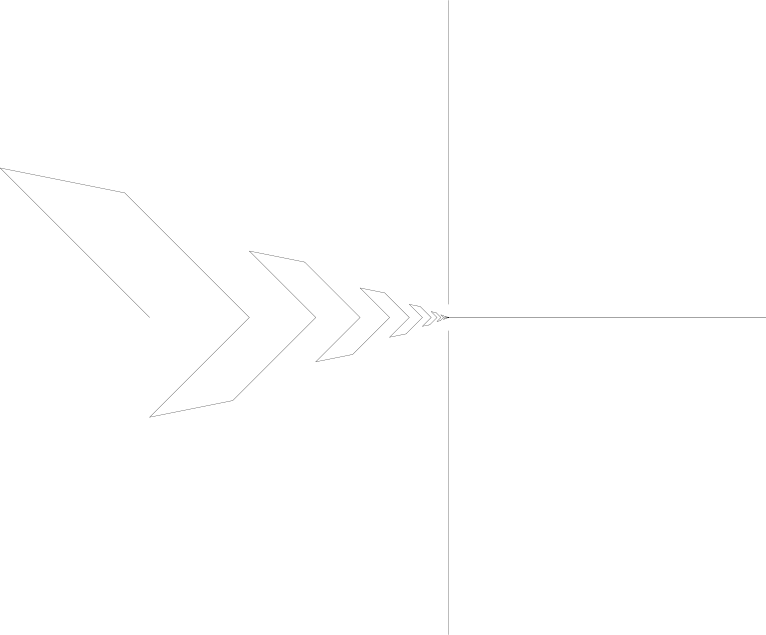
\includegraphics{\figdir/approach-pt.pdf}
    \caption{An example of a crossing and a $B_{\varepsilon}$ where
      $\forall \eta \in (0, \varepsilon)$, $K$ intersects
      $B_{\eta}(c_i)$ more than $4$ times.}
    \label{fig:approach-pt}
  \end{figure}
\end{remark}
\begin{proof}
  By definition of a discrete diagram, $c_i$ is an isolated point of
  the set of crossings, $\ms C$. Hence, there exists $\varepsilon > 0$
  such that $B_{\varepsilon}(c_i) \cap \ms C = \set{c_i}$.

  In general, we can have many arcs of $K$ contained in
  $B_{\varepsilon}(c_i)$; however, the definition of a discrete
  diagram stipulates only \emph{two} such arcs will be involved in the
  crossing itself (see \cref{fig:ex-b-veps}).
  \begin{figure}[H]
    \centering
    \hspace{-1cm}
    \includegraphics[scale=.7]{\figdir/extended-curves-on-circle.pdf}
    \caption{Example of $B_{\varepsilon}(c_i)$. The dashed lines show
      places where the strands poke outside $B_{\varepsilon}(c_i)$.
      Note, if being pedantic, the ball should be technically be
      centered on $c_i$.}
    \label{fig:ex-b-veps} % `example b varepsilon'
  \end{figure}
  % {\color{red} \huge Actually this is a diagram for $B_\eta$.}
  We'll
  take a somewhat funky notation here and use $\overleftarrow{A}$ to
  denote the preimage of the arcs in \cref{fig:ex-b-veps}.
  \[
    \overleftarrow{A} = K(S^1) \cap \fpre{\pi}{B_{\varepsilon}(c_i)}.
  \]
  We can visualize $\overleftarrow{A}$ by something like the
  following:
  \begin{figure}[H]
    \centering
    % \hspace{-2cm}
    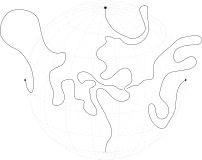
\includegraphics[scale=.8]{\figdir/extended-curves-on-sphere.pdf}
    \caption{Example $\protect\overleftarrow{A}$ in $\RR^3$, with a
      3-ball drawn to help communicate that we're no longer in
      $\RR^2$. Note that the dashed lines are \emph{not} included in
      $\protect\overleftarrow{A}$.}
  \end{figure}

  % In general, we \emph{don't} get $\overleftarrow{A}$ bound in a
  % 3-ball of radius $\varepsilon_i$. However, we can always bound
  % $\overleftarrow{A}$ in a cylinder of finite length. As it turns out,
  % this will be an extremely convenient way to complete the proof so
  % we'll do that in a moment. First, a word on notation: In the
  % following we'll use $C_i$ to denote a cylinder in $\RR^3$. This is
  % similar to (but unrelated with) the symbol $\ms C$ we used for the
  % set of all crossings of our diagram; the reader should try not to
  % confuse them.

  Without loss of generality, suppose our projection $\pi$ was onto
  the $xy$ plane. We want to show that $\overleftarrow{A}$ is bounded
  in the $z$ direction. To that end, note that $K$ is a continuous
  function from a compact space, hence it is bounded. This gives us
  $\overleftarrow{A}$ is bounded, hence there exists $r_\varepsilon >
  0$ such that $\overleftarrow{A} \subseteq \ol{B_{\varepsilon}(c_i)}
  \times [-r_\varepsilon, r_\varepsilon] $. Call this cylinder
  $C_\varepsilon$.
  \[
    C_\varepsilon = \ol{B_{\varepsilon}(c_i)} \times [-r, r].
  \]
  \begin{figure}[H]
    \centering
    \includegraphics[scale=.5]{\figdir/extended-curves-r3.pdf}
    \caption{An example drawing for $C_\varepsilon$}
  \end{figure}

  % WLOG, suppose $c_i = (0,0)$ and that $\pi$ was the projection onto
  % the $xy$ plane.\footnote{We do this just so that we can write the
  %   description of the cylinder cleanly. Note, rotations and
  %   translations are ambient isotopies on $\RR^3$, so this causes no
  %   problems.} It follows that $\overleftarrow{A}$ is bounded the
  % closed cylinder $C_i = \ol{B_{\varepsilon_i}(c_i)} \times [-2r,
  % 2r]$.\footnote{We need to take $2r$ in case the strands passes
  %   through $(0,0,0)$ and is one of the points realizing the diameter
  %   $r$.}

  We now have a claim. Essentially, it states that if we look at a
  sub-cylinder $C_\eta$ that's small enough, there are only finitely
  many points where our strands intersect the boundary. This will be
  important when we construct an ambient isotopy to remove them later.
  Note, there is nothing special about using $c_i$ defined in the
  following claim. The same should hold for any point in $\RR^3$.

  \begin{leftbar}

    \noindent \textbf{Claim 1:} There exists $\eta, r_\eta > 0$ such
    that $\eta < \varepsilon$, $r_\eta < r_\varepsilon$, and $C_\eta$
    defined by % and only
    % finitely many arcs of $\overleftarrow{A}$ intersect the cylinder
    \[
      C_\eta = \ol{B_{\eta}(c_i)} \times [-r_\eta, r_\eta].
    \]
    is such that $\partial C_\eta \cap \overleftarrow{A}$ is finite.
    % In particular, $C_\eta$ contains the strands yielding the crossing
    % $c_i$ in our diagram.

    \noindent \textbf{Proof of Claim 1:} We show existence for $\eta$;
    the existence of $r_\eta$ follows similarly.

    % \begin{enumerate}
    %   \item Suppose that the strand goes along
    % \end{enumerate}



    % To argue the part about
    % $C_\eta$ containing the strands from the crossing, observe that
    % \np{the contradiction we derive in the proof below works taking
    % $\varepsilon_1 = \varepsilon_i$ (for the $r'$ argument,
    % analogously $r' = r$)} and argue that the crossing strands
    % aren't a proper subset of $\partial C_i$.

    Suppose, to obtain a contradiction, that no such $\eta$ exists.
    One can show that this requires the strand to oscillate infinitely
    (think wiggly-feral point), per the following sketch: The only
    other way the claim could occur would be if for each $\eta$, there
    were a strand going around part of the circumference of
    $B_\eta(c_i)$. One can show that each such strand has nonzero
    length, and that this causes problems with the fact that there are
    infinitely-many $\eta$ (we'd end up filling a portion of the
    region).

    Let $\eta_0, \eta_1 \in (0, \varepsilon]$ with $\eta_0 \neq
    \eta_1$; without loss of generality suppose $\eta_0 < \eta_1$. By
    hypothesis, infinitely many arcs $\set{A_j}_{j \in J}$ of
    $\overleftarrow{A}$ intersect both of the cylinders.
    \[
      C_{\eta_0} = B_{\varepsilon_0}(c_i) \times [-r_\varepsilon,
      r_\varepsilon] \qquad\qquad \qquad\qquad C_1 = B_{\eta_1}(c_i)
      \times [-r_\varepsilon, r_\varepsilon].
    \]
    This might look something like the following:
    \begin{figure}[H]
      \centering
      \begin{subfigure}[t]{.49\linewidth}
        \centering
        \includegraphics[scale=.5]{\figdir/countably-intersecting-cylinder.pdf}
      \end{subfigure}~
      \begin{subfigure}[t]{.49\linewidth}
        \centering
        \includegraphics[scale=.6]{\figdir/countably-intersecting-cylinder-td.pdf}
      \end{subfigure}
      \caption{An example visualization in 3D showing the top strand
        of the crossing, another arc, and the bottom strand of the
        crossing, each separated vertically. The projection obtained
        is shown at the bottom, and the corresponding top-down view
        displayed on the right.}
      \label{fig:example-3d-oscillation-visual}
    \end{figure}
    We want to show this breaks continuity of $K$. To that end, we'll
    employ sequential continuity. First, we define a collection of
    sub-strands that live in the annulus between $\eta_0$ and $\eta_1$:
    For all $j\in J$, let
    \[
      B_j =
      \begin{cases}
        A_j \cap \ol{C_{\eta_1} - C_{\eta_0}} & \text{if } \abs{A_j
          \cap C_{\eta_0}} = 1 = \abs{A_j \cap C_{\eta_1}}, \text{ and }\\
        \varnothing & \text{otherwise}.
      \end{cases}
    \]
    Note that the $B_j$ omit the arcs that just oscillate around one of
    $\partial C_{\eta_0}$, $\partial C_{\eta_1}$ without ever going over
    to the other.

    To ensure the $B_j$ are actually valid arcs, we must subdivide them
    into their maximal connected components and remove all of the empty
    entries. Reindex the $B_j$ accordingly to yield $\set{B_\ell}_{\ell
      \in L}$. Then define sets $\set{O_\ell}_{\ell \in L}$,
    $\set{I_\ell}_{\ell \in L}$ ($O$ for ``outer'', $I$ for ``inner'')
    by for all $\ell \in L$,
    \[
      O_\ell = B_\ell \cap \partial C_{\eta_1}
      \qquad\qquad\text{and}\qquad\qquad I_\ell = B_\ell \cap \partial
      C_{\eta_0}.
    \]
    Let $\pn{O_{n}}{n \in \NN}$ be an arbitrary sequence of distinct
    $O_{\ell}$'s. Note that $C_{\eta_1}$ is compact, thus we can apply
    Bolzano-Weierstrass to $\set{O_{n}}_{n \in \NN}$ to obtain a
    convergent subsequence $\set{O_{n_k}}_{k \in \NN}$. Now, observe
    that because the $O$'s are endpoints of arcs bridging $\partial
    C_{\eta_0}$, $C_{\eta_1}$, each $O_{n_k}$ has a corresponding
    $I_{n_k} \in \partial C_{\eta_0}$. Apply Bolzano-Weierstrass to
    $\set{I_{n_k}}_{k \in \NN}$ to get \emph{another} convergent
    subsequence, call it $\pn{I_{n_m}}_{m \in \NN}$. Note that
    restricting the $O$'s to $\pn{O_{n_m}}_{m \in\NN}$ still yields a
    convergent sequence.

    Now, recall that because $K$ is an embedding, it is a homeomorphism
    onto its image. Thus, image and preimage under $K$ preserve
    convergence, and so taking the elementwise inverse of the $O_{n_m}$,
    $I_{n_m}$ gives us sequences in
    \[
      \set{\ms O_{n_m}}_{m \in \NN} \qquad\qquad \text{and} \qquad\qquad
      \set{\ms I_{n_m}}_{m \in \NN}
    \]
    in $S^1$. One can show that they must converge to the same $s \in
    S^1$ as follows: Observe each arc $A_{n_m}$ linking $O_{n_m}$,
    $I_{n_m}$ corresponds to an interval of one of the forms
    \[
      \sbk{\ms I_{n_m}, \ms O_{n_m}} \qquad\qquad\text{or}\qquad\qquad
      \sbk{\ms O_{n_m}}, \ms I_{n_m}.
    \]
    Since $S^1$ is compact, in order for these intervals to be disjoint
    (required since the images are disjoint) the lengths must go to $0$
    as $m \to \infty$. Thus $\ms O_{\ell_m} \to \ms I_{\ell_m}$.

    But note, taking the image once more gets us that $K(\ms O_{\ell_m})
    = O_{\ell_m} \not \to I_{\ell_m} = K(\ms I_{\ell_m})$ (since the
    $O_{\ell_m}$, $I_{\ell_m}$ are separated by $\eta_1 - \eta_0$). But
    this is a contradiction (\jiong), $K$ preserves convergence. Thus,
    there must exist $\eta > 0$ such that only finitely many of the arcs
    of $\overleftarrow{A}$ intersect $B_\eta(c_i) \times \RR$. Applying
    a similar argument for $r_\eta$ gives us the existence of the
    desired $C_\eta$, which proves the claim. \hfill $\square$

  \end{leftbar}
  % \hrulefill
  \begin{figure}[H]
    \centering
    \includegraphics[scale=.5]{\figdir/extended-curves-r3-two-cylinders.pdf}
    \caption{An attempted drawing of $C_\varepsilon$ and $C_\eta$.
      % Unfortunately, the opacity stacking didn't quite work out, so
      % some portions of the ball / strands got occluded when they
      % shouldn't have been.
    }
    \label{fig:the-cylinders}
  \end{figure}
  \begin{remark}
    Note that in the particular example shown in
    \cref{fig:the-cylinders}, we could have just taken $\eta =
    \varepsilon$. An example of when we can't is when one of the
    strands travels in a circular arc partway around $\partial
    C_\varepsilon$.
  \end{remark}


  OK: By the claim, there exists $\eta$, $r_\eta > 0$ such that
  \[
    \eta \in (0, \varepsilon) \qquad\qquad \text{and} \qquad\qquad
    r_\eta \in (0,r_\varepsilon)
  \]
  and $\overleftarrow{A}$ intersects $\partial C_\eta = B_{\eta}(c_i)
  \times [r_\eta, r_\eta]$ at finitely-many points. Apply the claim a
  second time to define a proper sub-cylinder $C_\nu$ by $C_\nu =
  B_{\nu}(c_i) \times [-r_\nu, r_\nu]$ (where $\nu < \eta$ $r_\nu <
  r_\eta$) such that $\overleftarrow{A}$ only intersects $C_\nu$ at
  finitely-many points.


  The next claim essentially states that we can remove \np{the strands
    that don't participate in our crossing} from $C_\nu$ by pushing
  them out into $C_\eta$. Note, the fact that we have only
  \emph{finitely} many points of intersection helps in avoiding an
  appeal to
  \cref{thm:uniformly-convergent-ambient-isotopy}.\footnote{There is a
    more direct proof using the techniques of
    \cref{sec:rigorous-ambient-isotopy}, but it's horrible to write
    out formally.}

  % {\color{red} \Large Wait there's some more stuff to consider. The
  %   proof I gave was for oscillatory behavior, but that might not be
  %   where the problems lie. Really it's in the garbage w' having
  %   circumference strands??????????????/}

  % an
  % appeal to \cref{thm:uniformly-convergent-ambient-isotopy} (uniform
  % convergence \& ambient isotopy).

  \begin{leftbar}
    \textbf{Claim 2:} Let $S_o, S_u$ be the strands corresponding to
    the overstrand and understrand (respectively) in
    \cref{fig:ex-b-veps}. Let $\set{S_j}_{j =1}^{n}$ be the collection
    of arcs of $\overleftarrow{A}$ that intersect $C_\eta$ but
    \emph{do not} participate in the crossing. Then we can find an
    ambient isotopy $F : [0,1] \times C_\eta \to C_\eta$ such that
    \begin{enumerate}
      \item $F$ keeps \np{both the boundary of $C_\eta$
        \emph{and} the crossing strands $S_o$, $S_u$} fixed, and
      \item For all $x \in S_j$, $F(1, x) \in C_\eta \setminus
        C_\nu$ ($F$ moves all the other strands outside $C_\nu$).
    \end{enumerate}

    \textbf{Proof of Claim 2:} Observe that for each $j=1,\ldots, n$,
    $\partial T_j$ yields a crossing-less curve. Thus, one can apply
    \cref{prop:replacing-by-same-endpoints} to find ambient isotopies
    moving each into $C_\eta \setminus C_\nu^\circ$, keeping the rest
    of the region fixed. Since we have only finitely-many strands to
    remove, concatenating them yields another ambient isotopy. \hfill
    $\square$
    % Consider the following ambient isotopy on $\RR^2$: each of the
    % $M_\mu$ gets sent to the corresponding part of the circumference
    % bordered by $R_\mu$, and each of the displayed portions of the
    % circumference get sent to the \emph{dotted} lines shown. Finally,
    % the rest of the ambient space we're displacing gets squished into
    % the region bounded by the dashed lines, which stay fixed (as do
    % the crossing strands themselves).
    % \footnote{This can be justified
      % by applying \cref{thm:same-region-ambient-isotopic} to each of
      % the finitely-many strands on }


  \end{leftbar}

  One way to visualize the net effect of this process is as follows.
  Note that the crossing strands (marked with the black dots in
  \cref{fig:part-disjoint-regions}) partition $B_{\eta}(c_i)$ into
  four disjoint regions $R_1, R_2, R_3, R_4$ that contact $\partial
  B_{\nu}(c_i)$. Let $M_1, M_2, M_3, M_4$ be defined by for each index
  $\mu \in \set{1,2,3,4}$, $M_\mu = \partial R_\mu$.

  \textbf{Note:} In the figures below, we accidentally re-drew
  $B_\nu(c_i)$ as $B_\varepsilon(c_i)$, and $B_\eta(c_i)$ as some ball
  containing $B_\varepsilon$. We apologize for this inconsistency;
  unfortunately, we currently do not have enough time to go back and
  fix them.
  \begin{figure}[H]
    \centering
    \includegraphics{\figdir/extended-curves-on-circle-partition.pdf}
    \caption{The regions $R_1, R_2, R_3, R_4$, and (approximations
      of) the corresponding $M_1, M_2, M_3, M_4$'s in black. Not to
      scale.}
    \label{fig:part-disjoint-regions}
  \end{figure}
  Then we ``push'' $\partial R_\mu \cap \partial \ol{B_\nu(c_i)}$
  outwards to the dotted curves shown below, and $\partial R_\mu \cap
  B_\nu(c_i)$ out to the circumference. The dashed lines (representing
  $\partial B_\eta(c_i)$) remain fixed.
  \begin{figure}[H]
    \centering
    \includegraphics[scale=.9]{\figdir/extended-curves-on-circle-ms-isotopy.pdf}
  \end{figure}
  Finally: observe that by construction,
  \begin{enumerate}
    \item $C_\nu \subsetneq C_\eta \subsetneq C_\varepsilon$,
    \item $\abs{F(1, K) \cap \partial\bk{\fpre{\pi}{B_\nu(c_i)}}} =
      \abs{F(1,K) \cap \partial C_\nu} = \abs{\set{\text{endpoints of
      $S_o, S_u$}}} = 4$, and
    \item $\partial C_\varepsilon$ remains fixed.
  \end{enumerate}
  As desired.
\end{proof}
\begin{corollary}[$K$ can be polygonalized near crossings]
  Let $K$, $c_i$, $C_\nu$, $C_\varepsilon$ be as defined in the
  preceding theorem/proof. Then there exists an ambient isotopy $F :
  [0,1] \times \RR^3 \to \RR^3$ such that
  \begin{enumerate}
    \item $F$ is identity outside of $[0,1] \times C_\varepsilon$, and
    \item $F(1, K) \cap C_\varepsilon$ is polygonal.
  \end{enumerate}
\end{corollary}
\begin{sproof}[Sketch]
  By the \cref{thm:cleaning-up-near-crossings}, we can find an ambient
  isotopy removing all non-crossing strands from $C_\nu$ while keeping
  $\partial C_\varepsilon$ and \np{the crossing strands themselves}
  fixed. Apply this ambient isotopy from $t = 0$ to $t= 1/2$. Then,
  \begin{itemize}
    \item Observe that there are no other strands in $\fpre{\pi}{B_\nu(c_i)}$
      ``above'' $S_o$ or ``below'' $S_u$.
    \item Use this to define an ambient isotopy flattening out $S_o$
      in the $z$ direction (so that it's only non-polygonal in $x$ and
      $y$), while translating it half of the way to the top circular
      cap of $C_\nu$. Apply a similar ambient isotopy flattening $S_u$
      out in $z$ and moving it half of the way to the bottom circular
      cap.\footnote{Although drawn for a different purpose,
      \cref{fig:example-3d-oscillation-visual} displays this idea
      nicely the blue/red circles. Note, there we drew the crossing
      strands as straight lines in $xy$ as well as in $z$; we have not
      done this yet in our construction.}
    \item Use a proof similar to that of
      \cref{prop:replacing-by-same-endpoints} (taking a smaller
      sub-cylinder if necessary) to turn the crossing strands into
      straight lines while keeping $\partial C_\nu$ fixed.
  \end{itemize}
  This yields the desired result.
\end{sproof}
Finally, this concludes the analysis of behavior near crossing points.
We are now ready to put it all together.

\section{The Conclusion}

Together, these give us the following theorem:
\begin{theorem}[Discrete Diagram Implies Countably
  Polygonal]\label{thm:discrete-diagram-countably-polygonal}
  Let $K : S^1 \into \RR^3$ be a knot. Then if $K$ admits a discrete
  diagram $D$, then $K$ is ambient isotopic to a knot comprised of (at
  most) a countable union of polygonal segments.
\end{theorem}
\begin{proof}
  Apply \cref{thm:cleaning-up-near-crossings} to triangulate $K$ at
  each of the crossing points. Note that this implicitly defines a
  collection of pairwise-disjoint arcs connecting each of the
  resulting $C_\nu$ together. Applying
  \cref{cor:full-polygonalizing-strands}, we can polygonalize each of
  these connecting strands with a finite collection of line segments.

  Finally, observe that for each crossing, this gives us a finite
  collection of corresponding polygonal segments. By
  \cref{prop:at-most-countable-crossings}, we have at most
  countably-many crossings in the diagram, hence the total number of
  polygonal segments employed is at most countable!
\end{proof}
The following appears to be a reasonable extension of the claim.
\begin{conjecture}
  If the set of wild points are topologically discrete, then the same
  result as above holds.
\end{conjecture}
% \begin{sproof}
%   $\msf{K}{S^1}$ is compact, hence a discrete subset
% \end{sproof}

% A couple of other results also follow from patching together parts of
% the arguments above:
The techniques above can be used to obtain a variety of other expected
results. E.g.,
\begin{proposition}
  Let $K_0, K_1 : S^1 \into \RR^3$. Suppose that the diagrams for
  $K_0$, $K_1$ are related by planar isotopy. Then $K_0 \cong K_1$.
\end{proposition}
In particular:
\begin{corollary}
  Let $K_0, K_1 : S^1\into \RR^3$ such that $K_0$, $K_1$ share the
  same discrete diagram $D$. Then $K_0 \cong K_1$.
\end{corollary}
We conclude this section with a discussion of directions for future
work.


\subsection{A Generalization of Reidemeister's Theorem?}
The usual proof of Reidemeister's theorem relies on using
polygonalizations to reduce the problem of ambient isotopy to the
elementary moves. Now that we have a locally-polygonal representation
for some wild knots, can we prove an analogous theorem for countable
sequences of moves? E.g., something like
\begin{conjecture}
  Let $K_0, K_1 : S^1 \into \RR^3$ be knots with discrete diagrams.
  Suppose that $K_0 \cong K_1$. Then there exists a sequence of
  Reidemeister moves satisfying the hypotheses of
  \cref{thm:uniformly-convergent-ambient-isotopy} taking $K_0$ to
  $K_1$.
\end{conjecture}
One plan of attack might be as follows:
\begin{enumerate}
  \item \cref{thm:uniformly-convergent-ambient-isotopy} (or
    alternatively, \cref{thm:countable-gluing-ambient-isotopies})
    gives us an ``if'' direction (provided we're careful to mind
    bijectivity in the
    \cref{thm:uniformly-convergent-ambient-isotopy} case). Hence,
    the main plan of attack would be to find an only-if proof.
  \item One idea could be as follows: First, show that given an
    ambient isotopy $F : [0,1] \times \RR^3 \to \RR^3$ taking
    $K_0$ to $K_1$, we can realize the same effects on $K_0$,
    $K_1$ by restricting $F$ to a compact subspace $V$. Then use
    this to argue that $F$ restricted to $F : [0,1] \times V \to
    V$ is uniformly continuous. Hence, we can partition $[0,1]
    \times V$ into a finite collection of small sub-regions such
    that $F$ is guaranteed to vary by less than $\varepsilon$ on
    them.
  \item First, note that the local sets we constructed in the
    proof in the previous section (e.g., the $C_\nu$, or the sets
    guaranteed by \cref{thm:separating-strands}) can be made
    arbitrarily small. Use this to argue that our choices of
    polygonal representatives can be made continuously dependent
    in some sense on the input knots themselves.
  \item Then, show that in light of the above, away from wild
    points, we can realize the effects of the ambient isotopy
    by local polygonal moves. Near the wild points, keep the
    effect of the given $F$.
  \item Define a uniformly convergent sequence of ambient
    isotopies ``shrinking'' the region where we keep the effects
    of $F$ down to the wild points. Finally, apply
    \cref{thm:uniformly-convergent-ambient-isotopy} to yield the
    result.
\end{enumerate}




% \begin{sproof}

% \end{sproof}

% We have a couple of remarks:
% \begin{remark}
%   Observe that all of the sets we employed ($B_\varepsilon(c_i)$, the
%   $V$'s from \cref{thm:separating-strands}, etc) can all be made
%   arbitrarily small, which allows us to make our polygonalization
%   ``continuously'' dependent on the input knot in some sense.
% \end{remark}
% \begin{remark}
%   By applying \cref{thm:discrete-diagram-countably-polygonal}, one can
%   argue that
% \end{remark}


% \begin{proposition}

% \end{proposition}









%%% Local Variables:
%%% TeX-master: "../../kobayashi-thesis"
%%% End:
